\chapter{User Experience und Kriterien}
\label{Kapitel:UX}
In diesem Kapitel werden die Unterschiede aber auch die Gemeinsamkeiten und Übereinstimmungen von User Experience und Usability herausgearbeitet. Es werden Kriterien beschrieben, durch die die User Experience beeinflusst wird und Evaluationsmethoden hierfür angegeben.


%Der Begriff User Experience ist aus dem Bereich der Usability erwachsen

%User Experience und Usability sind voneinander abhängig. 


%Nur wenn ein Nutzer sich in einem System wohl fühlt, kann er auch gut damit arbeiten. Auf der anderen Seite muss er mit einem System gut arbeiten können, damit er sich darin wohl fühlt. 

%Im letzten Jahrzehnt ist der Begriff User Experience, kurz UX, ein Modewort im Bereich der Mensch-Computer-Interaktion geworden. Das hängt damit zusammen, dass die Technologien sich interaktive Techonlogien stark weiterentwickelt haben und somit nicht nur praktischer und leichter benutzbar geworden sind, sondern auch mit der Mode gehen und auch oft wie eine besondere Art Modeobjekt gesehen werden. Dies steht im Kontrast zur Vergangenheit, in der besagte Technologien eher als Werkzeuge angesehen und  eingesetzt wurden.\\
%Der Begriff der UX wurde in verschiedenen Fachkreisen schnell aufgenommen, wird aber an vielen Stellen als ungenau oder schwer definierbar betitelt. 
%Eine weit gefasste Definition wäre UX als den Bereich zwischen Nutzbarkeit und positiven bzw. negativen Gefühlen bei Benutzung einer Technologie beschrieben. 
%\cite{Forlizzi:2004dz} \\
%Im Laufe der Zeit hat sich die Bedeutung des Begriffs UX, nach Meinung einiger Experten, sogar als Gegenbewegung zur vorherrschenden Usability entwickelt. Usability fokussiert im Gegensatz zur User Experience, wie bestimmte Aufgaben leichter bewältigt werden können.
%Eine frühe Definition von UX setzt das Erlebnis einer Person in dem Moment, in dem es erlebt wird in den Mittelpunkt. Produktivität und Erlernbarkeit stehen dabei klar im Hintergrund.\\
%\\
%\cite{Hassenzahl:2011ju}



\section{Entwicklung des Begriffs User Experience}
\label{Anschnitt:EntwicklingUX}
Im letzten Jahrzehnt ist der Begriff User Experience, kurz UX, häufig im Bereich der Mensch-Computer-Interaktion diskutiert worden. Dabei wurden die Erlebnisse und die damit verknüpften Emotionen eines Benutzers im Hinblick auf die von ihm benutzten Systeme erörtert und in den Vordergrund gestellt. Zuvor wurde primär die Benutzerfreundlichkeit (engl. \textit{usability}) von Softwareoberflächen betrachtet. Dies hatte das Ziel den Benutzer eines Systems bei der Arbeit zu unterstützen, damit er seine Aufgaben schneller und leichter bewältigen kann. \cite[S. 23f.]{Nielsen:1994vk}  \\
Anfänglich konnte die Usability eines Systems bzw. einer Software nicht genau bestimmt werden \cite[S. 23f.]{Nielsen:1994vk}. Auf Grund dessen wurden drei Kriterien standardisiert, mit denen sich die Benutzerfreundlichkeit messen lässt. Das erste Kriterium ist die Effektivität und bezieht sich darauf, wie genau und vollständig ein Benutzer eine Aufgabe vollenden kann. Das zweite Kriterium ist die Effizienz, es gibt an mit wie viel Aufwand eine Aufgabe im Hinblick auf Genauigkeit und Vollständigkeit fertiggestellt werden kann. Das letzte Kriterium greift die Zufriedenheit des Anwenders auf. Es überprüft die positive Einstellung des Nutzers gegenüber des Systems und ob es von ihm ohne Unbehagen einsetzbar ist.
\cite{DIS:3VJ9kaCr}
Die Eigenschaften des dritten Kriteriums, der Zufriedenheit, zielen auf die Emotionen des Benutzers ab und stellen somit die Verbindung zur User Experience her.
Die Betrachtung der Gefühle der Benutzer ist mit der Entwicklung neuer interaktiver Technologien einher gegangen. Auf der einen Seite hat sich der Formfaktor der Hardware verkleinert während die Leistungsfähigkeit vergrößert wurde, auf der anderen Seite wurde der Mensch und seine Emotionen bei der Entwicklung immer stärker in den Mittelpunkt gestellt. Aus diesem Zusammenhang stammt der Begriff User Experience Design, kurz UXD. \glqq \textit{Die Idee von User Experience Design ist es also, das Erlebnis des Kunden ins Zentrum der Produktentwicklung zu stellen und dem Kunden möglichst viele positive Erlebnisse mit dem Produkt zu bieten.}\grqq\ \cite[S. 3]{Moser:2012cn} \\
Abschließend lässt sich sagen, dass es eine Vielzahl an Beschreibungen für den Begriff User Experience gibt, aber eine konkrete Definition noch aussteht \cite[S. 4]{Bernhaupt:2010vi}. Erschwerend hinzu kommen die Überschneidungen mit dem Fachbereich der Usability.







%Als weitere Kriterien werden Erlernbarkeit, Einprägsamkeit und Fehleranfälligkeit genannt[S. 26ff.]{Nielsen:1994vk}. Durch diesen flexiblen Kriterienkatalog ist eine klare Trennung der User Experience von der Usability nicht möglich.

%Es ist schwierig eine konkrete Definition für den Begriff User Experience zu geben . 
%Im Kontext der User Experience beschreibt das Wort \glqq Experience\grqq\ somit nicht Erfahrungswerte, sondern Erlebnisse und zielt auf die damit verknüpften Emotionen ab. Für Emotionen und Gefühle gilt dasselbe wie für den Begriff User Experience, es sind Worte, die alltäglich benutzt werden aber nur schwer zu definieren sind. Jeder Mensch ist täglich verschiedenen Emotionen ausgesetzt, daher glauben viele Menschen zu wissen, was Emotionen sind. Auch hier ist die genaue Definition schwierig.
% \glqq Everyone knows what an emotion is, until asked to give a definition\grqq\ \cite[S. 464]{Fehr:1984hm}\\
% Ein Punkt in dem die Wissenschaftler übereinstimmen ist, dass Emotionen ein facettenreiches Themengebiet sind, in denen Phänomene, wie Körpersprache, Gesichtsausdrücke, Gemütszustände und innere Bewältigungsstrategien behandelt werden.
% Daher gibt es auch keine feste Richtlinie, nach der sich Emotionen auswerten lassen.\cite[S. 28]{Zimmermann:2006uv}
% (Gerade im Hinblick auf Videospiele müssen Emotionen genauerer betrachtet werden, da hier gezielt Spannung, Freude und Trauer erzeugt werden soll, im Gegensatz zu einer Anwendungssoftware)





\section{User Experience und Usability}
\label{Abschnitt:BegriffsdefinitionUX}
Einen genauen Unterschied zwischen User Experience und Usability festzusetzen und zu beschreiben ist nicht möglich. Im vorherigen Abschnitt \ref{Anschnitt:EntwicklingUX} wurde beschrieben, wie sich der Begriff User Experience im Bereich der Usability entwickelt hat. Dies geht soweit, dass User Experience sogar als Gegenbewegung zur Usability gesehen wird \cite[S. 91]{Hassenzahl:2011ju}. 
Im Laufe dieser Entwicklung haben sich drei verschiedene Ansichten herauskristallisiert, die versuchen das Zusammenspiel von User Experience und Usability zu beschreiben.
%Die Grenzen und Definitionen von User Experience und Usability sind nicht klar abgesteckt somit sind die Übergänge an einigen stellen fließend. (Evtl. Henne-Ei-Problem anmerken?) Es kristallisieren allerdings drei unterschiedliche Standpunkte heraus, die klar voneinander abgegrenzt sind. 
\\ 
Der erste Standpunkt sieht die User Experience als einen allumfassendes Themengebiet an. In ihm ist die User Experience ein weit gefächertes Konzept, das neben anderen Aspekten auch den Bereich Usability enthält. Im Vordergrund steht die Interaktion des Benutzers mit dem System bzw. der Software und was er während der Zeit der Benutzung empfindet. Die Grundlagen für diese hervorgerufenen Emotionen werden aber schon vor Erwerb des Produktes gelegt und auch andere Bereiche, wie z.B. der Support beeinflussen was ein Benutzer empfindet. \cite[S. 10f.]{Folstad:2006uh}\\
Der zweite Standpunkt fasst User Experience und Usability als gleichwertige Themengebiete auf. Bei diesem Standpunkt wird nur der Zeitrahmen der Benutzung eines Produktes betrachtet. Im Bereich der UX werden hier die emotionalen und experimentellen Aspekte fokussiert. Zusätzlich fallen auch weitere Teilaspekte die der Usability zugeschrieben werden in den Bereich der User Experience. Ein Beispiel hierfür ist die Fehleranfälligkeit \cite[S. 26]{Nielsen:1994vk}, wodurch es beim Nutzer zu Frustration kommen kann. \cite[S. 10f.]{Folstad:2006uh} \\
Der dritte und letzte Standpunkt sieht die User Experience als einen Aspekt der Usability. Wie in Abschnitt \ref{Anschnitt:EntwicklingUX} beschrieben sind die Hauptkriterien von Usability Effizienz, Effektivität und Zufriedenheit. Bei diesem Ansatz beschränkt sich der Bereich der User Experience auf den Faktor Zufriedenheit. Auch hier wird nur die Nutzungsdauer des Produktes betrachtet. \cite[S. 10f.]{Folstad:2006uh}
\\
Der Kontext dieser Arbeit steht vor dem Hintergrund des ersten Standpunktes. Das Thema User Experience wird als ein allumfassendes Oberthema gesehen. Der Fokus liegt dabei auf der Nutzung der Software, im Fall dieser Arbeit auf dem Spielen eines Videospiels. 

%In Videospielen rückt die Usability in den Hintergrund. Jedoch kann dieses nicht in voller Breite beschrieben werden. Daher liegt der Fokus auf der Erarbeitung von Kriterien für eine positive User Experience, die sich auf das Spielen eines Videospiels beziehen.



%    klIn der Mensch-Technik Interaktion wird "User Experience" (Nutzungserleben) oft recht eng     als eine vom Produkt ausge- löste Bewertung des Benutzers verstan- den. Den Begriffen „Erleben“ und "Er- lebnis" wird diese Sichtweise nicht ge- recht, geht es doch dabei vielmehr um die Verknüpfung von Handeln, Fühlen, und Denken (in der Interaktion mit einem Produkt) zu einem Ganzen. "Experience Design" setzt sich nun zum Ziel, Erlebnisse gezielt zu schaffen (oder zumindest zu ermöglichen). Im Zent- rum steht also das zu gestaltende Er- lebnis und nicht mehr das Produkt. Dadurch ergibt sich eine Reihe von Herausforderungen an "experience design" und Gestalter. Zwei davon, nämlich die Kluft zwischen Bedürfnis und Produkt und die Rolle des zukünf- tigen Benutzers, werden diskutiert.


%Zunaechst sind Erlebnisse per Definition subjektiv. Sie spielen sich \glqq im Kopf\grqq\ der Benutzer ab, die damit zum eigentlichen Qualitaetsmassstab werden. Gebrauchs- tauglichkeit wurde lange und wird auch heute noch als etwas Objektives ver- standen. Es geht eben eher um die Effi- zienz an sich als um ein Effizienzerleben (was sich auch trotz objektiv niedriger Effizienz einstellen kann, da objektive Merkmale und subjektives Erleben nur lose gekoppelt sind). Erleben ist also ein psychologisches Phaenomen, allerdings eben nicht im Sinne eines spezifischen psychologischen Prozesses, sondern als die unteilbare Repraesentation gerade bewusster Prozesse und Inhalte.


%McCarthy und Wright (2004) benennen vier unterscheidbare \glqq Faeden\grqq\ der Erle- bens: das Sinnliche, dass Emotionale, das Raeumlich-zeitliche und das \glqq Zusammengesetzte\grqq\. Die ersten beiden betonen die Zentralitaet der Sinne und des Fuehlens; die letzten beiden betonen die Unteilbarkeit eines Erlebnisses und ganz besonders seine Dynamik (z.B. Karapanos et al., 2009). Natuerlich sind die Sinne und das Fuehlen untrennbar verknuepft mit Denken und Handeln. Er- leben kann also als eine Art innerer Kommentar verstanden werden – ein kontinuierlicher Strom aus Denken, Handeln, Fuehlen und Bewerten. Wird dieses Erleben zu einer in sich ge- schlossenen, bedeutungsvollen Episode zusammengefasst, entsteht ein Erlebnis (vgl. Forlizzi und Battarbee, 2004). Solche Erlebnisse geben unseren Handlungen Bedeutung, sie werden erinnert, kom- muniziert und wirken motivierend (oder abschreckend). Und natuerlich koennen interaktive Produkte eine Rolle in diesen Erlebnissen spielen: als Ausloeser oder Verstaerker des Erlebens.




\section{Kriterienkatalog} 
\label{Abschnitt:Kriterienkatalog}
Neben der unklaren Definition des Begriffes User Experience gibt es auch keine standardisierten Kriterien, um die User Experience eines Systems zu ermitteln. Unter Zuhilfenahme einer Usability Evaluationen lässt sich aber ein Kriterienkatalog herleiten. Als Basis für den Kriterienkatalog dient eine Studie von Nike, in der die Usability der hauseigenen Fußball Webseite, Nike-Football, evaluiert wurde. In dieser Studie hat ein Großteil der männlichen Probanden die Webseite gut bewertet, obwohl sie die einzelnen Usability Kriterien schlecht bewertet haben. Folglich muss es weitere Kriterien geben, die Einfluss auf die Wahrnehmung des Nutzers haben. \cite[S. 69f.]{Hartmann:2006vx}\\
In einer anschließenden Befragung stellte sich heraus, dass eingeblendete Videos zu diesem Ergebnis führten. Die Probanden antworten \glqq I would have to say it’s great just because I liked these videos so much\grqq\ \cite[S. 71]{Hartmann:2006vx} oder ähnliches. In den Videos wurden spannende Fußballszenen dargestellt.\\ 
%In einer von Nike durchgeführten Studie, in der die Usability der hauseigenen Fußball Webseite, Nike-Football, evaluierte wurde, stellte sich heraus, dass auf Grund eingeblendeter Videos ein Großteil der männlichen Probanden die Webseite als gut bewertete. In diesen Videos wurden  Fußballspieler gezeigt, die diverse Tricks mit Fußbällen vollführten. \glqq I would have to say it’s great just because I liked these videos so much\grqq\ \cite[S. 71]{Hartmann:2006vx}. \\ 
%Im Widerspruch dazu steht, dass zuvor ein Großteil der selben Probanden die Usability der Webseite negativ bewertet hat. Folglich muss es weitere Kriterien geben, die nicht zu den klassischen Usability Kriterien aus Abschnitt \ref{Anschnitt:EntwicklingUX} gehören und trotzdem Einfluss auf die Wahrnehmung des Nutzers haben. \\
Testpersonen, die sich in ihrer Bewertung nicht auf die Videos bezogen, haben die Webseite sowohl positiv als auch negativ bewertet, ohne dabei gezielt auf spezielle Merkmale der Webseite einzugehen. Bei einer anschließenden gezielten Nachfrage konnten sie ihre Bewertung nicht genau begründen. Ein Teil der Befragten bezog sich auf Aspekte, wie das Aussehen der Webseite oder einzelne Punkte aus dem Usability Katalog. Andere gaben an, dass sie nach Bauchgefühl bewertet haben oder zogen andere Webseiten zum Vergleich heran. Wieder andere gaben an, dass sie dem Thema Fußball in Gänze zu- bzw. abgeneigt sind. \cite[S. 71]{Hartmann:2006vx}\\
Durch die Auswertung der Antworten der Probanden ist folgender Kriterienkatalog zur User Experience entstanden. \\
\begin{description} 
\item[Marke/Identität] ist das erste Kriterium dieses Katalogs. Schon im Vorfeld wird hierdurch unterbewusst bestimmt was ein Nutzer bei Erstkontakt mit einem System oder einer Software empfindet \cite[S. 12 \& S. 17f.]{Gutjahr:2013gi}. 
Im Zusammenhang mit der von Nike durchgeführten Evaluation steht das Image der Firma Nike, aber auch das Verhältnis des Nutzers zum Fußball. Hat der Nutzer schon vorab positive oder negative Erfahrungen mit der Firma oder deren Produkten gehabt hat, dies auf seine Bewertung einen Einfluss. Selbiges gilt für das Thema Fußball. \cite[S. 71]{Hartmann:2006vx} 
\item[Ästhetik] im Bezug auf die Nutzeroberfläche ist das zweite Kriterium. Es ist der erste direkte Berührungspunkt eines Nutzers mit einem System. Dieses Kriterium beherbergt zum einen Bedienelemente, wie Buttons, Scrollbars und viele weitere, zum anderen aber auch Bilder, Audioelemente und Videos. Diese multimedialen Elemente haben eine direkte Verbindung zum Gemütszustand des Benutzers. Im Englischen wird dieses Kriterium daher treffender als \glqq Look and Feel\grqq\ bezeichnet. \\
Es wurde festgestellt, dass Bilder aus der Natur oder Landschaftsaufnahmen einen beruhigenden Einfluss auf den Betrachter haben. Bilder mit technologischem Hintergrund wie z.B. Autos, Smartphones, Hardwarekomponenten wecken die Neugier und wirken somit stimulierend \cite[S. 2]{Sutcliffe:2002fs}. Da es sich bei einem Firmenlogo auch um ein Bild handelt, kann es an genau dieser Stelle zu Überschneidungen zwischen dem ersten und zweiten Kriterium kommen. Auf einer Webseite wird für gewöhnlich das Logo der jeweiligen Firma abgebildet und auch in Betriebssystemen wie Windows oder MacOS befindet sich das Firmenlogo in der Menü- bzw. Taskleiste. Abgesehen vom ersten Kriterium gibt es zusätzlich noch weitere Berührungspunkte mit anderen Kriterien. \cite[S. 71]{Hartmann:2006vx}
\item[Usability] ist das dritte Kriterium. Es umfasst alle Unterpunkte, Effektivität, Effizienz und Zufriedenheit, die in Abschnitt \ref{Anschnitt:EntwicklingUX} beschrieben wurden. Dieses Kriterium kann in Abhängigkeit zum zweiten Kriterium der Ästhetik stehen. Der Zusammenhang liegt in den Bedienelementen. So können graphisch veränderte Buttons einen Nutzer irritieren, so dass es ihm schwer fällt im System zu navigieren. \cite[S. 71]{Hartmann:2006vx}
\item[Personalisierungs-/Anpassungsmöglichkeit] ist ein weiteres Kriterium, das in Verbindung mit der Ästhetik eines Systems steht. Neben dem Erscheinungsbild kann es auch in Zusammenhang mit der Usability stehen. Da flexible Systeme dem Nutzer die Bedienung erleichtern, lassen sich Aufgaben schneller und leichter erledigen. Als Beispiel hierfür dient die Möglichkeit Schriften größer darzustellen. \cite[S. 72]{Hartmann:2006vx}
Hierdurch wird das Lesen und somit die Usability erleichtert, auf der anderen Seite kann es aber dazu kommen, dass Texte unscharf oder verpixelt dargestellt werden, in anderen Fällen können sie auch über Bildschirm Begrenzungen herausragen. Dies sollte im Rahmen des Ästhetik Kriteriums unterbunden werden.\\
\item[Inhalt \& Funktionsumfang]ist das letzte Kriterium. Gerade bei Webseiten ist es wichtig die Inhalte so zu strukturieren, dass sie einfach vom Nutzer aufgenommen werden können. Neben den Inhalten werden den Besuchern einer Webseite im Regelfall weiterführende Funktionalitäten an die Hand gegeben. Dies könnte z.B. die Möglichkeit sein einen Artikel in einem Webshop zu kaufen. Dabei kann die Realisierung dieses Beispiel-Shops weitere Funktionalitäten bieten, wie die Möglichkeit Artikel auf eine Merkliste zu setzen oder Bewertungen für Artikel zu verfassen. \cite[S. 71]{Hartmann:2006vx}
\end{description}
Insgesamt wurden fünf verschiedene Kriterien auf Basis des Usability-Tests ausgearbeitet, die direkten Einfluss auf die User Experience haben. In Abbildung \ref{pic:UXJudgement} werden diese Kriterien grafisch dargestellt. Zusätzlich wird gezeigt mit welchen Kriterien die Ästhetik in Verbindung steht.
\begin{figure}[H]
    \centering
    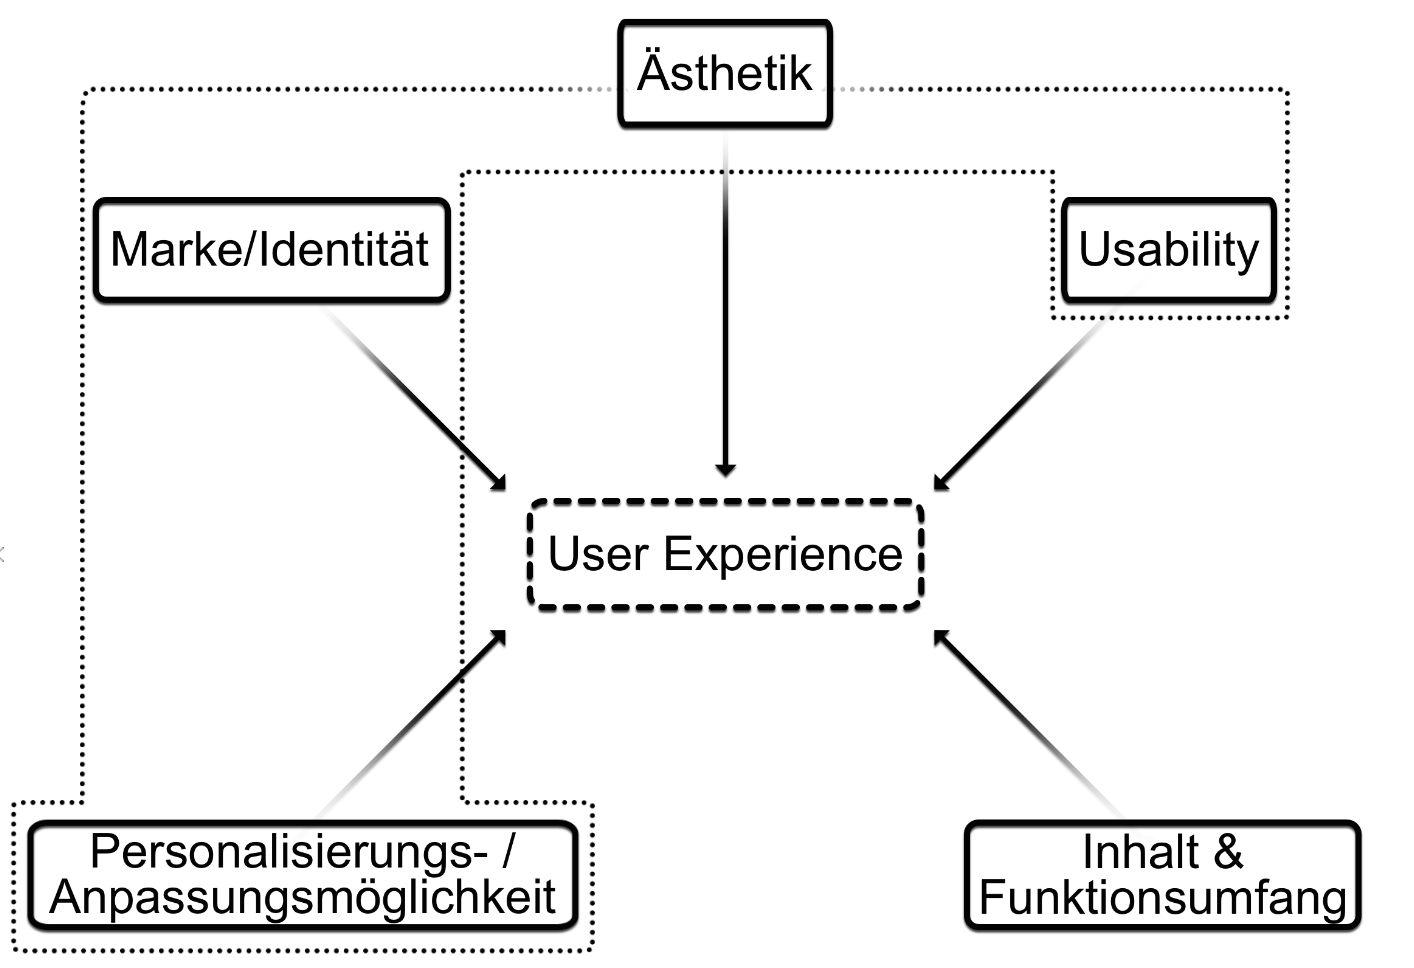
\includegraphics[width=.8\textwidth]{files/ux/judgement}
    \caption{Kriterien der User Experience vgl. \cite[S. 71]{Hartmann:2006vx}}
    \label{pic:UXJudgement}
\end{figure}
Um eine gute User Experience in einem System zu gewährleisten, können diese Kriterien mittels unterschiedlicher Methoden schon während der Entwicklung geprüft werden.


%
%Zur Überleitung evtl.
%b
%Page 158
%In classical usability evaluation, the ‘task’ is a crucial issue.
%
%Defining and Measuring User Experience:
%Are They Two Sides of the Same Coin?
%Jan Stage




\section{Methoden zur Evaluation der User Experience} 
\label{Abschnitt:MethodenEvaluationUX}


%
%Erst Emotionen Kategorisieren:
%Im Umgang mit UX sind die Teilbereiche Affekt, Emotion und Stimmung wichtig, da diese gut ausgewertet werden können.
%\cite[S. 28]{Zimmermann:2006uv}
%
%
%ear, happiness, sadness, anger, indignation, contempt, contentment, pride, envy, love, hate, surprise, disgust, nostalgia, melancholy, satisfaction, and many more. Diverse writers have proposed that there are from two to twenty of these “basic emotions”
%
%Empirical research seems to converge toward a two- dimensional structure of core affect. It is proposed that core affect, at any slice in time, can be described by two independent dimensions, degree of pleasantness (valence) and degree of activation (arousal). 
%

Die Auswertung der in Abschnitt \ref{Abschnitt:Kriterienkatalog} definierten Kriterien lässt sich mit Hilfe verschiedener Methoden bewerkstelligen. Der Ursprung dieser Methoden liegt im Bereich der Usability, daher muss sichergestellt werden, dass die zuvor definierten Kriterien in jede Methode einfließen. Des Weiteren muss bei der Wahl der jeweiligen Methode der Entwicklungsstand des zu prüfenden Systems beachtet werden, da sich die Methoden in Aussagekraft und Effizienz unterscheiden. So sollten zu Beginn der Entwicklung effiziente Methoden gewählt werden, um den Entwicklungsprozess nicht zu verlangsamen. \cite[S. 224]{Moser:2012cn}
\begin{description} 
\item[Hallway Test] 
 - Die schnellsten Ergebnisse, ohne lange Vorbereitungszeit, liefert der Hallway Test. Bei dieser Methode werden Arbeitskollegen zu einem oder mehreren Kriterien befragt. Vor Beginn dieses Tests muss kurz erläutert werden, welche Inhalte geprüft und welche Aufgaben bewältigt werden sollen. Die Fragestellungen hierfür müssen im Vorfeld so präzise ausgearbeitet sein, dass dem Probanden während der Bearbeitung keine weiteren Hinweise zur Bewältigung der Aufgaben gegeben werden müssen. Jeder Eingriff des Aufgabenstellers kann die Qulität der späteren Auswertung verringern. Analysiert werden bei diesem Test die Gedankengänge des Probanden. Daher muss die Testperson während des gesamten Tests möglichst genau beschreiben, an was sie im jeweiligen Moment denkt. Um genauere Ergebnisse zu erzielen sollte derselbe Test mit mehreren Mitarbeitern durchgeführt werden. Bei den zusammengetragenen Ergebnissen muss zudem beachtet werden, dass es sich bei den Probanden weder um spätere Anwender des Systems noch um User Experience Spezialisten handelt. Somit ist die Aussagekraft der Ergebnisse eingeschränkt. \cite[S. 226]{Moser:2012cn}
\item[Pluralistic Walkthrough] 
 - Eine erweiterte Variante des Hallway Tests ist der Pluralistic Walkthrough. Bei diesem Test werden neben den Programmierern auch spätere Anwender des zu entwickelnden Systems mit einbezogen. Dies geschieht in Form eines Workshops, für den im Vorfeld Aufgaben definiert wurden. Nach einer kurzen Einleitung, die die Nutzer mit dem System bekannt machen sollen, werden im ersten Schritt die zuvor definierten Aufgaben von den Anwendern bearbeitet. Um eine Beeinflussung untereinander zu verhindern, müssen die Probanden getrennt von einander arbeiten. Im Gegensatz zum Hallway Test dürfen die Probanden bei dieser Methode aber Fragen stellen, sollten sie eine Aufgabe nicht bewältigen können. Im Anschluss daran wird im Plenum eine Musterlösung der Entwickler vorgestellt. Darauf folgen die Nutzer mit der Präsentation ihrer Ergebnisse. Nachdem alle Ergebnisse präsentiert worden sind diskutieren zunächst nur die Anwender die unterschiedlichen Herangehensweisen. Die Entwickler werden in diesem Schritt bewusst nicht berücksichtigt, damit sie nicht mit ihrem Hintergrundwissen die Gedankengänge der Nutzer beeinflussen. Zum Abschluss des Workshops werden dann die Entwickler in die vorherige Diskussionsrunde mit einbezogen. \cite[S. 228f.]{Moser:2012cn}
\item[Cognitive Walkthrough] 
 - Eine andere Methode, um im frühen Entwicklungsstadium einen Prototypen zu testen ist der Cognitive Walkthrough. Bei diesem Ansatz versuchen sich einer oder mehrere Experten aus dem Bereich User Experience in die Rolle eines Anwenders hineinzuversetzen und die zuvor festgelegten Aufgaben zu bewältigen. Dies geschieht unter der Annahme, dass ein Nutzer immer die naheliegendste Lösung wählt. Zusätzlich muss der Experte die Absichten des Anwenders verstehen oder zumindest kennen, um so Bedienungsabläufe möglichst realitätsnah durchführen zu können. Hauptsächlich wird dadurch die Nutzeroberfläche auf ihre Benutzbarkeit untersucht, dazu gehören sowohl GUI-Elemente als auch die Anzahl an Schritten, die benötigt werden eine Aufgabe zu lösen. \cite[S. 234f.]{Moser:2012cn}
\item[Heuristische Evaluation] 
 - Eine ähnliche Herangehensweise bietet die heuristische Evaluation. Bei dieser Methode wird ein System basierend auf Erfahrungswerten von Experten getestet. Sowohl beim Cognitive Walkthrough als auch bei der heuristischen Evaluation steigt die Qualität des Ergebnis mit der Anzahl der Spezialisten. Zusätzliche können spätere Anwender mit einbezogen werden. Dies wirkt sich ebenfalls positiv auf die Qualität aus, da konstruierte Arbeitsabläufe immer fehleranfällig sind. Die entsprechenden Evaluationen lassen sich auch an Hand von Prototypen durchführen und können somit bereits in frühen Entwicklungsstadien eingesetzt werden. Hierfür existieren Heuristiken die je nach Projekt angepasst und erweitert werden können. \cite[S. 232f.]{Moser:2012cn}\\
Folgende Heuristiken wurden von Jakob Nielsen aufgestellt:
\begin{itemize}
\item Ist die Nutzeroberfläche aufgeräumt und leicht verständlich?\\
Fälschlicher Weise wird häufig angenommen, dass durch zusätzliche Funktionalitäten und Optionen mehr Nutzer zufrieden gestellt werden können. Die graphische Nutzeroberfläche eines Systems sollte so einfach wie möglich gestaltet werden. Jede Information und jede Option muss vom Nutzer aufgenommen und verstanden werden, somit ist jedes Element eine zusätzliche Fehlerquelle. Im Idealfall werden dem Nutzer zu jedem Zeitpunkt nur die Elemente angezeigt, die er gerade benötigt. Um dieses Ziel weitestgehend zu erreichen sollten Aufgabenanalysen durchgeführt werden.\\
Bedienelemente und Arbeitsabläufe sollten realitätsnah gestaltet werden. Ein Beispiel hierfür ist der \glqq Papierkorb\grqq\ , der in vielen Betriebssystemen zum Löschen von Dateien benutzt wird. Zum einen sieht das Symbol aus wie ein handelsüblicher Papierkorb, zum anderen entspricht der Ablauf des Wegwerfens und des endgültigen Entleerens dem Arbeitsablauf in der Realität.\\
Elemente müssen unter Anwendung der Gestaltgesetze logisch gruppiert werden. Diese Gesetzte besagen, dass Elemente die 
einen geringeren Abstand zueinander haben, die dieselbe Farbe haben, die miteinander verbunden sind oder die von einem Rahmen umschlossen werden als zusammengehörend wahrgenommen werden. \\
Farben sind sparsam einzusetzen, denn eine Nutzeroberfläche sollte unabhängig von den Farben verwendet werden können. Sie sollten nur zum  Kategorisieren oder Hervorheben gebraucht werden. Zudem müssen sie sich eindeutig voneinander unterscheiden um Verwechslungen zu verhindern. Quantitative Informationen sollten generell nicht durch Farben dargestellt werden. So ist es möglich farbblinden Nutzern die Bedienung des Systems zu erleichtern.\cite[S. 115 ff.]{Nielsen:1994vk} %TODO

\item Ist die Terminologie an den Benutzer angepasst? \\
Die Dialoge eines Systems sind in der Muttersprache des Benutzer zu verfassen. Dies bezieht sich nicht nur auf die einzelnen Wörter, sondern auch auf Symbole, die in verschiedenen Kulturkreisen unterschiedliche Bedeutungen haben können. Ein Nutzer sollte nicht mit systeminternen Bezeichnungen (Variablen oder deren Typ) in Berührung kommen. So sollen Währungen in einer Finanzsoftware beispielsweise nicht durch schwer erkennbare Codes sondern ausgeschrieben, als Abkürzung oder Symbol, dargestellt werden. \cite[S. 123 ff.]{Nielsen:1994vk}

\item Wird das Gedächtnis des Nutzers nicht zu stark beansprucht?\\
Eine auf einem Computer gespeicherte Information verändert sich nicht, sie wird immer exakt gleich ausgegeben. Nur wenige Menschen haben ein fotographisches Gedächtnis. In der Regel sind Erinnerungen ungenau und/oder lückenhaft. Durch Hinweise in Form von  Texten und Symbolen können Erinnerungen genauer abgerufen werden. Dies lässt sich umsetzen indem Eingabefeldern Beispiele hinzugefügt werden. So muss ein Benutzer nicht darüber nachdenken in welcher Form ein Datum eingeben werden muss. Selbiges gilt auch für komplexere Aufgaben. \cite[S. 129 ff.]{Nielsen:1994vk}
% Je nach Umfang können Gedächtnisstützen auch in Form von Symbolen oder Zeichnungen dargestellt werden. 
%Aus ähnlichen Gründen wird in der Sprachwissenschaft wird zwischen aktivem und passivem Wortschatz unterschieden.

\item Ist das System konsistent? \\
Konsistenz ist einer der wichtigsten und offensichtlichsten Punkte. Gleiche Aufgaben sollten immer mit der gleichen Herangehensweise gelöst werden können. Wenn ein Nutzer einen Befehl oder einen Arbeitsablauf gelernt hat, sollte er diesen auch bei weiterführenden oder ähnlichen Aufgaben anwenden können. Dies führt dazu, dass sich ein Nutzer das Gefühl bekommt ein System zu beherrschen. Die Eigeninitiative des Nutzers wird gefördert. Er kann das Gelernte immer wieder anwenden und so ihm auch noch unbekannte Funktionalitäten erschließen. \cite[S. 132 f.]{Nielsen:1994vk}

%Hinzu kommt, dass die Eigeninitiative des Nutzers gefördert wird, was dazu führt das ein Nutzer das gelernte auch an anderen Stellen anwendet und sich somit wiederum selber weiterbilden kann. %Consistency is one of the most basic usability principles. If users know that the same command or the same action will always have the same effect, they will feel more confident in using the system, and they will be encouraged to try out exploratory learning strate- gies because they will already have part of the knowledge needed to operate new parts of the system . 

\item Erhält der Nutzer direktes Feedback durch das System?\\
Mit Feedback ist in diesem Zusammenhang nicht die Rückmeldung von Fehlern gemeint, sondern das Ausgeben von Informationen zum aktuellen Systemstatus und Hinweisen zu den Eingaben eines Nutzers. Dieses Feedback sollte innerhalb eines Zeitfensters von einer bis zehn Sekunden geschehen. Bei längeren Wartezeiten kann es dazu kommen, dass ein Nutzer die Rückmeldung mit einer nicht relevanten Aktion verknüpft. Eine Autovervollständigung von Adressdaten oder die Einblendung einer Uhr, bei Wartezeiten können hierfür als Beispiel angeführt werden. %The system should continuously inform the user about what it is doing and how it is interpreting the user's input. Feedback should not wait until an error situation has occurred: The system should also provide positive feedback, and it should provide partial feed- back as information becomes available. For example, the way to write the German letter ii on many keyboards involves first typing the umlaut, .., and then typing the character that is to go under the two dots. Some systems provide no visible feedback as the first part of the character is typed, leading many novice users to conclude that the system does not know how to deal with umlauts. A better design would show the umlaut and then change the cursor in some way to indicate that the system was waiting for the second part of the character. 10 seconds is about the limit for keeping the user's attention focused on the dialogue. For longer delays, users will want to perform other tasks while waiting for the computer to finish, so they should be given feedback indicating when the computer expects to be done. Feedback during the delay is especially important if the response time is likely to be highly variable, since users will then not know what to expect. 
\cite[S. 134 ff.]{Nielsen:1994vk}


\item Kann das System unkompliziert beendet werden?\\
Jeder Dialog sollte mit einem Button zum Schließen, Beenden oder Abbrechen versehen sein. Ist dies nicht der Fall kann es passieren das sich Nutzer in einem System gefangen fühlen. Es ist darauf zu achten, dass bei einem Abbruch das System in den vorherigen Status zurückgesetzt wird. Wurde eine Datei fälschlicher Weise bearbeitet, sollte durch einen Abbruch die ursprüngliche Datei wiederhergestellt werden. %Users do not like to feel trapped by the computer. In order to increase the user's feeling of being in control of the dialogue, the system should offer the user an easy way out of as many situations as possible. For example, all dialog boxes and system states should have a cancel button or other escape facility to bring the user back to the previous state. In many cases, exits can be provided in the form of an undo facility that reverts to the previous system state [Abowd and Dix 1992; Yang 1992].Users quickly learn to rely on the existence of undo, so it should be made pervasively available throughout the system as a generic command that undoes any state changes rather than being restricted to only undoing a special category of user actions.
\cite[S. 138 f.]{Nielsen:1994vk}

\item Kann ein Nutzer Shortcuts verwenden?\\
Shortcuts sind da, um Arbeitsabläufe für fortgeschrittene Nutzer zu verkürzen. Dazu gehören Tastenkürzel wie \textit{\glqq CTRL+P\grqq}, mit dem sich eine Datei ausdrucken lässt, aber auch anpassbare Dialoge, die es ermöglichen bestimmte Funktionalitäten schneller zu erreichen. Ein System muss auch ohne Shortcuts vollständig bedienbar sein. %Even though it should be possible to operate a user interface with the knowledge of just a few general rules, it should also be possible for the experienced user to perform frequently used operations especially fast, using dialogue shortcuts. Typical accelerators include abbreviations, having function keys or command keys that package an entire command in a single keypress, double-clicking on an object to perform the most common operation on it, and having buttons available to access important functions directly from within those parts of the dialogue where they may be most frequently needed. Pen computers, vertual realities, and some mouse interfaces may may also use gestures as accelerators. Type-ahead (typing the next input before the computer is ready to accept it) is not really a shortcut as such since it still requires the user to generate a complete sequence of input, but it can speed up the interaction by allowing the user to get ahead of the computer and not have to pay attention to all the steps in the dialogue. 
\cite[S. 139 ff.]{Nielsen:1994vk}

\item Gibt es aussagekräftige Fehlermeldungen? Wird der Arbeitsablauf durch sie nicht gestört? \\
Der Moment in dem ein Fehler auftritt ist eine Schlüsselsituation. Auf der einen Seite kann der Nutzer seine Aufgabe nicht wie gewünscht vollenden, auf der anderen Seite hat der Nutzer in dieser Situation die Möglichkeit ein System besser kennenzulernen. Durch die Unterbrechung seines Arbeitsablaufes ist er in einem Zustand gesteigerter Aufmerksamkeit. Deshalb sollten Fehlermeldungen so formuliert sein, das der Benutzer sie schnell und gut verstehen kann. Fehlermeldungen in Form von unlesbaren Codes, die erst in Handbüchern oder im Internet nachgeschlagen werden müssen, sind zu vermeiden.\\
Bei der Formulierung ist darauf zu achten, das der Nutzer nicht beschuldig wird. Anschuldigungen führen nur zu Verunsicherung. Daher ist \glqq ILLEGAL USER ACTION, JOB ABORTED\grqq\ (\cite[S. 143]{Nielsen:1994vk}) eine schlechte Fehlermeldung. Außerdem ist es wichtig in so einer Situation die Informationen des Systems mit einzubeziehen, um möglichst detaillierte Fehlermeldungen auszugeben. In komplizierteren Fällen kann es nötig sein, dass dem Nutzer lange Fehlermeldungen mit weiterführenden Informationen angezeigt werden müssen. In solchen Fällen bieten sich mehrstufige Fehlermeldungen an. Das bedeutet, dass anfangs nur ein kleiner Abriss der Fehlermeldung angezeigt wird und der Nutzer aktiv weiter durch die Fehlermeldung navigieren kann.  \\
Tritt ein Fehler auf, sollte er den Arbeitsfluss so gering wie möglich beeinflussen. Ein System sollte so konstruiert sein, dass es nach einem Fehler nicht \textit{terminiert} und somit den Nutzer nicht dazu zwingt seinen Arbeitsvorgang zu wiederholen. Stattdessen sollten Nutzer in der Lage sein, einzelne Schritte rückgängig zu machen, um so Fehler zu korrigieren oder zu vermeiden. \cite[S. 142 ff.]{Nielsen:1994vk}

%1. Problem für den User, er kann sein Aufgabe nicht lösen.
%2. Der User hat hier eine Möglichkeit das System besser kennenzulernen. 
%Der User ist aufmerksamer, und kann durch leichter lernen.
%Dem liegen einige Informationen zu Grunde, aus denen Sinnige Fehlermeldungen konstruiert werdern können.

%Fehler melden sollten klar und deutlich formuliert sein. User sollte nicht mit fehlercodes konfrontiert werden. So das er die fehlermeledung verstehen kann ohne in Handbüchern oder sonstigen verzeichnissen nachschlagen muss.


%Sie sollten präzise formuliert sein. datei xy kann nicht geöffnet werden, da keine entsprechnede anwendung installiert ist. 
%Dies kann errreicht werden in dem man versucht zu konstruieren, was ein nutzer machen wollte. 
%Sollten aber auch so formuliert sein, das der Nutzer nicht in irgendeiner form beschuldigt wird. 
%Sie sollten auch nicht zu stark in den Vordergrund gestellt werden

%"ILLEGAL USER ACTION, JOB ABORTED" (\cite[S. 143]{Nielsen:1994vk}) < worst

%Instead of putting all potentially useful bits of information in all messages, it is possible to use shorter messages that will be faster to read as long as the user is given easy access to a more elaborate message. The most common way to implement multilevel messages is to have only two levels and to supplement the short initial message with a button that can be clicked for more inform



%Error situations are critical for usability for two reasons: First, by definition they represent situations where the user is in trouble and potentially will be unable to use the system to achieve the desired goal. Second, they present opportunities for helping the user understand the system better [Frese et al. 1991] since the user is usually motivated to pay some attention to the contents of error messages, and since the computer will often have some knowledge of what the problem is. They should be phrased in clear language and avoid obscure codes. It should be possible for the user to understand the error message by itself without having to refer to any manuals or code dictionaries. They should be precise rather than vague or generaL For example, instead of saying, "Cannot open document the computer should say "Cannot because the application is following the principle about giving feedback by restating the user's input).
%One useful way of generating constructive error messages is by guessing at what the user really meant to say. In the case of textual input, spelling-correction methods have been available for many years [Peterson 1980;Bentley 1985],and these methods can be especially fast and precise wh
%Finally, error messages should be polite and should not intimi- date the user or put the blame explicitly on the user. Users feel bad enough as it is when they make errors. There is no need for the computer to make the situation even worse by accusing error messages like the classic "ILLEGAL USER ACTION, JOB ABORTED" (in upper case, at that-screaming at the user). 
%In addition to having good error messages, systems should also provide good error recovery. For example, users should be allowed to undo the effect of erroneous commands, and they should be able to edit and reissue previous commands without having to enter them from scratch.



\item Wird Fehlern vorgebeugt?\\
Noch wichtiger als gut verständliche Fehlermeldungen ist es, Situationen zu erkennen in denen häufig Fehler entstehen können. Jede Eingabe eines Nutzers ist eine potentielle Fehlerquelle. Werden diese Eingaben validiert, bevor sie vom System verarbeitet werden, lässt sich diese Fehlerquelle minimieren. Beispiele hierfür sind Rechtschreibfehler, die im Vorfeld korrigiert werden können aber auch die Eingabe eines Datums. Gerade bei Datumsangaben gibt es eine Vielzahl von Formatierungsmöglichkeiten. Monate können als Zahlen oder Worte eingegeben werden. Die Zahlen wiederum können mit Punkten oder Bindestrichen getrennt werden. Eine Alternative diesen Fehlern vorzubeugen ist es den Nutzer nicht direkt seine Daten eingeben zu lassen, sondern ihn aus einem Menü wählen zu lassen.\\
Ein anderer Weg der Fehlervorbeugung ist es ein System mit verschiedenen Modi auszustatten. Diese könnten ein Bearbeitungs-, ein Experten- und ein Präsentationsmodus sein. Im Bearbeitungsmodus erhält der Nutzer die Möglichkeit Daten zu erstellen und anzupassen. Im Expertenmodus könnte die Zugriffssteuerung für diese Daten geregelt werden und der Präsentationsmodus gibt die Daten geordnet und nicht editierbar aus. Unterschiedliche Modi bringen aber zusätzlich eine potentielle Fehlerquelle mit sich. Der Nutzer muss genau wissen, in welchem Modus er sich gerade befindet. Ist dies nicht schnell und leicht ersichtlich könnte er beispielsweise vergebens im Präsentationsmodus versuchen Daten zu bearbeiten. \cite[S. 145 ff.]{Nielsen:1994vk}

%Even better than having the good error messages recommended in the previous section would be to avoid the error situation in the first place. There are many situations that are known to be error- prone [Norman 1983;Reason 1990;Senders and Moray 1991],and systems can often be designed to avoid putting the user in such situations.

%For example, every time the user is asked to spell out something, there is a risk of spelling errors, so selecting a filename from a menu

%expert settings

\item Sind Hilfetext und weitere Begleittexte vorhanden?\\
Die meisten Nutzer lesen Handbücher und Begleittexte nicht. \glqq It is all explained in the manual\grqq\ \cite[S. 149]{Nielsen:1994vk} ist daher kein guter Leitsatz, wenn es zu Verständnisproblemen kommt. Wenn ein Nutzer ein System nutzt ohne sich eingelesen zu haben, kann es zu Situationen kommen in denen er vor einem scheinbar unlösbaren Problem steht und schnell Hilfe benötigt. Genau in dieser Situation greift er als erstes auf Hilfetexte und ähnliche Dokumente zu. Daher sollten diese im Vorfeld mit Bedacht gestaltet worden sein, damit ein Nutzer sein Problem möglichst schnell lösen kann. Es ist Sinnvoll diese Texte nicht nur in geruckter Form, sondern auch im Internet zu veröffentlichen, um den Zugriff und die Suche innerhalb der Texte zu vereinfachen.\cite[S. 148 ff.]{Nielsen:1994vk}


%"It is all explained in the manual" should never be the system designer's excuse when users complain that an inter- face is too difficult.

%The fundamental truth about documentation is that most users simply do not read manuals [Rettig 1991]. Users prefer spending their time on activities that make them feel productive [Carroll and Rosson 1987], so they tend to jump the gun and start using the system without having read all the instructions. If you doubt this common observation and think that your users do read the docu- mentation, try this simple experiment: visit a few users and place a 10 Dollar bill somewhere in their manuals. On your next visit, check how many of the bills are still there! (Of course, you can only use this technique once.)


%A corollary to this phenomenon is that if users do want to read the manual, then they are probably in some kind of panic and will need immediate help. This observation indicates the need for good, task-oriented search and lookup tools for manuals and online documentation. Since many users rarely use the manual before they absolutely have to, they may not have the manual immedi- ately available (it may have been lost or borrowed by another user), which is one reason for the trend toward supplementing printed manuals with online help and online documentation. 



\end{itemize}





%Heuristiken von Nielsen und Molich (1994)
%1. Ist der Systemstatus sichtbar?
%2. Stimmen System und reale Welt überein?
%3. Hat der Benutzer genügend Kontrolle und Freiheit?
%4. Ist die Lösung konsistent und hält Standards ein?
%5. Wird versucht Fehler zu vermeiden?
%6. Wird Erkennen Erinnern vorgezogen?
%7. Sind Abläufe flexibel und effizient?
%8. Ist das Design ästhetisch und minimalistisch?
%9. Gibt es Unterstützung bei Fehlern?
%10. Sind Hilfe und Dokumentation vorhanden?

%Heuristiken von Sarodnick und Brau (2006)
%1. Aufgabenangemessenheit
%2. Prozessangemessenheit
%3. Selbstbeschreibungsfähigkeit 
%4. Steuerbarkeit
%5. Erwartungskonformität
%6. Fehlertoleranz
%7. System- und Datensicherheit 
%8. Individualisierbarkeit
%9. Lernförderlichkeit
%10. Wahrnehmungssteuerung 
%11. Freude bei der Verwendung 
%12. Interkulturelle Aspekte

 
%Für jede Interaktion wird geprüft, ob alle Heuristiken eingehalten werden.  Verletzt ein Schritt eine Heuristik, wird dies als potentielles Usability-Problem no- tiert.  Oft braucht man dafür mehr als einen Durchgang.
%
%Nach der Einzeluntersuchung werden die Befunde zusam- mengetragen, besprochen und dokumentiert. Die einzel- nen Heuristiken werden dabei gerne für die Gruppierung der Befunde verwendet. Für jeden Befund wird ein Schwe- regrad abgeleitet, aus:
%􏰀 der Auftretenswahrscheinlichkeit
%􏰀 dem Grad der Beeinflussung
%􏰀 der Möglichkeit, das Problem zu umgehen.
%Der Schweregrad wird üblicherweise in einer Skala von 0-4 ausgedrückt (Nielsen, 1994):
%􏰀 0 = Kein Problem erkennbar 􏰀 1 = Reine Kosmetik
%􏰀 2 = Kleines Usability-Problem 􏰀 3 = Großes Usability-Problem 􏰀 4 = Fatales Usability-Problem 
% 
% 




%Form. USA
%Hierbei wird genauer betrachtet, wie Nutzer die zuvor gestellten Aufgaben lösen. Der Nutzer wird per Kamera beobachtet und der auch der Bildschirminhalt wird dem USA experten gezeigt. Der Nutzer ist während des Tests auf sich alleine gestellt, daher sollte der Test so ausführlich beschrieben sein, das keine Hilfe bei der Bewältigung der Aufgaben benötigt wird. Somit sollte diese Methode erst gegen Ende der Entwicklung stattfinden.
%
%Ablauf: Zu untersuchende Teile festelegen, Aufgaben formulieren nach Möglichkeit in ein Szenario einflechten, Aufgaben selber durchführen
%
%
\item[Formaler Usability-Test]
- In einem formalen Usability-Test wird das Verhalten eines Nutzers aufgezeichnet und analysiert, um zu erkennen wie gut ein Nutzer ein System bedienen kann. Die Abbildung \ref{pic:UsaTestAufbau} zeigt wie der Aufbau eines Usability-Tests ohne \glqq Eye-Tracking\grqq\ und weitere spezielle Sensoren aussehen könnte.\\
Einer Reihe von Nutzern werden verschiedenen Aufgaben gestellt, die sie mit Hilfe des Systems, unter Beobachtung lösen müssen. Nicht nur die einzelnen Arbeitsschritte werden aufgezeichnet sondern auch das Verhalten der Probanden. Die einzelnen Personen werden daher zusätzlich von einer Videokamera gefilmt. Alle Schritte, alle Bemerkungen und jegliches Zögern eines jeden Nutzers ist mit dem genauen Zeitpunkt zu protokollieren. Die Aufzeichnungen ermöglichen es gefundene Probleme im Nachhinein besser zu analysieren. \cite[S. 230f.]{Moser:2012cn} \\
Obwohl es sich um einen Usability-Test handelt lassen die Ergebnisse auch im Hinblick auf die User Experience auswerten. Viele Emotionen lassen sich am Gesicht eines Probanden ablesen. Auch Pulsmesser und weitere Sensoren können hierfür hinzugezogen werden. In einigen Fällen bietet es sich an die Bewegungen der Augen des Probanden aufzuzeichnen. Dieses Verfahren nennt sich \glqq Eye-Tracking\grqq\ . So lässt sich erkennen, welche Bildschirmbereiche der Nutzer stärker und welche er schwächer wahrnimmt. \\ 

\begin{figure}[H]
    \centering
    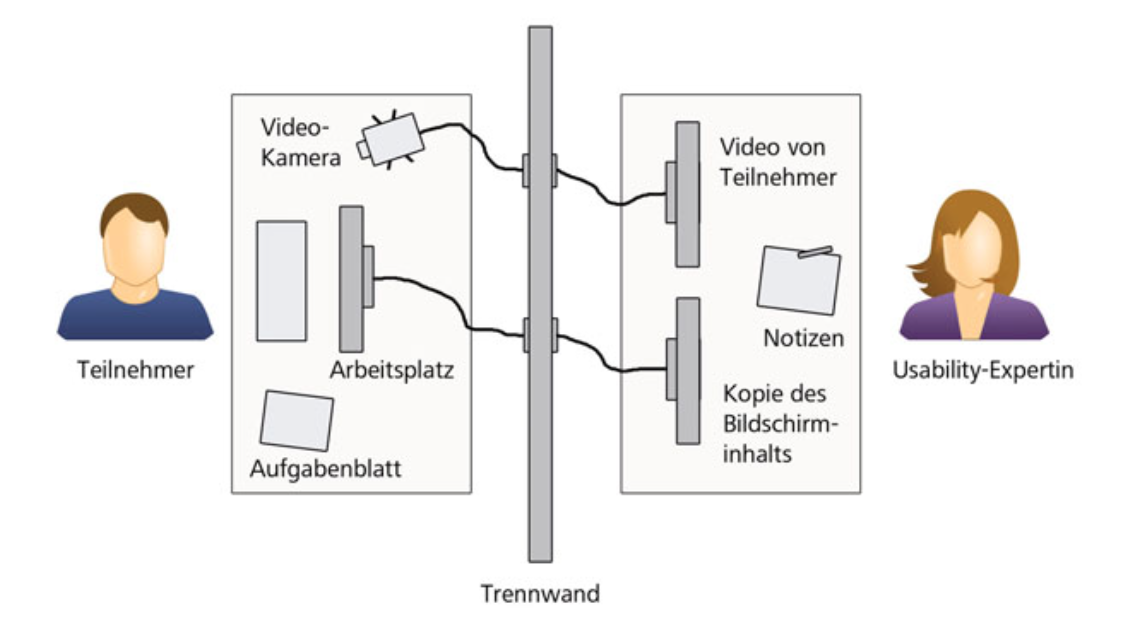
\includegraphics[width=.8\textwidth]{files/usa/aufbau}
    \caption{Der Aufbau eines Usablity-Tests. \cite[S. 230]{Moser:2012cn} }
    \label{pic:UsaTestAufbau}
\end{figure}


Ein Test dieser Art ist eine Stresssituation für den Nutzer, daher muss deutlich klar gemacht werden, dass es um den Test des Systems geht und keine Fehler beim Nutzer gesucht werden. Dem Nutzer die Möglichkeit zu geben den Test jeder Zeit abzubrechen kann den gefühlten Stress reduzieren.\\
Äußere Einflüsse müssen weitestgehend ausgeschlossen werden. Der Proband sollte also seine Aufgaben getrennt von den anderen Probanden und den Beobachtern bearbeiten. Damit die Probanden zu vergleichbaren und auswertbaren Resultaten kommen, ist es auch bei diesem Verfahren wichtig die gleichen Aufgaben zu stellen und diese schriftlich festzuhalten. Sie müssen dafür soweit ausgearbeitet sein, dass der Proband jede Aufgabe ohne weiteres Nachfragen bearbeiten kann. Idealerweise werden die Aufgaben hierfür in ein Szenario verpackt, um einen kompletten möglichst praxisnahen Arbeitsablauf zu testen. Der komplette Test sollte in einem Zeitfenster von einer Stunde bearbeitet werden können. Tests die länger dauern können durch Konzentrationsprobleme der teilnehmenden Personen verfälscht werden. Um dies zu ermöglichen, sollte der Test vor der Durchführung durchgespielt werden. Dabei sollten alle Fragen und Informationen auf Vollständigkeit, Verständlichkeit und Durchführbarkeit geprüft werden. \\
Auf Grund des Funktionsumfangs, das ein System benötigt, kann der formale Usability-Test erst mit einem fortgeschrittenen Prototypen oder in späteren Entwicklungsstadien durchgeführt werden. \cite[S. 230f.]{Moser:2012cn} \\
Je größer der Umfang eines Usability-Tests ist, desto höher sind die damit verbundenen Kosten. Die Kosten steigen jedoch nicht Proportional mit dem Nutzen. Es hat sich herausgestellt, das ein Test mit nur fünf Probanden einen Großteil der vorhandenen Probleme eines Systems aufdeckt. So liefert ein Test mit fünfzehn Nutzern deutlich weniger Einsicht, als ein gestaffelter Test mit jeweils fünf Nutzern in unterschiedlichen Entwicklungsstadien. Die Ursache hierfür liegt darin, dass offensichtliche Probleme in der Regel schon alleine von einem oder zwei Nutzern aufgedeckt werden. Jeder weitere Nutzer deckt weniger individuelle, noch nicht erfasste Probleme auf. In Abbildung \ref{pic:UsaTesters} wird dieses Verhältnis dargestellt. \cite{Nielsen:uc}


%The most striking truth of the curve is that zero users give zero insights.
%
%As soon as you collect data from a single test user, your insights shoot up and you have already learned almost a third of all there is to know about the usability of the design. The difference between zero and even a little bit of data is astounding.
%
%When you test the second user, you will discover that this person does some of the same things as the first user, so there is some overlap in what you learn. People are definitely different, so there will also be something new that the second user does that you did not observe with the first user. So the second user adds some amount of new insight, but not nearly as much as the first user did.
%
%The third user will do many things that you already observed with the first user or with the second user and even some things that you have already seen twice. Plus, of course, the third user will generate a small amount of new data, even if not as much as the first and the second user did.
%
%As you add more and more users, you learn less and less because you will keep seeing the same things again and again. There is no real need to keep observing the same thing multiple times, and you will be very motivated to go back to the drawing board and redesign the site to eliminate the usability problems.
%
%After the fifth user, you are wasting your time by observing the same findings repeatedly but not learning much new.



\begin{figure}[H]
    \centering
    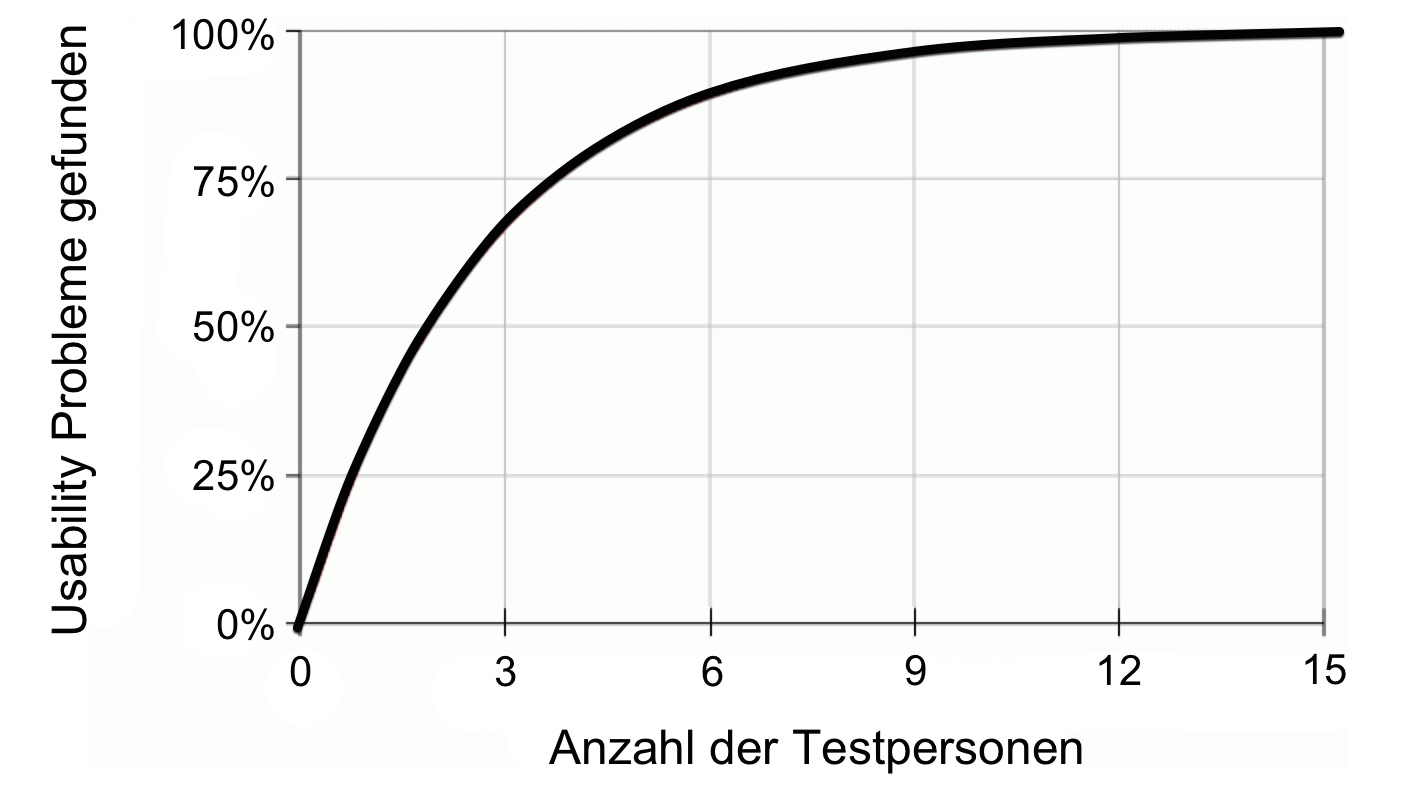
\includegraphics[width=.8\textwidth]{files/usa/anzahlTester}
    \caption{Verhältnis zwischen gefunden Usability Problemen und der Anzahl der Tester vgl. \cite{Nielsen:uc}}
    \label{pic:UsaTesters}
\end{figure}
 
% akribisch auf jeden Schritt, jede Bemerkung, jedes Zögern und jede Mausbewegung des Teilnehmers.
 
% Da dies eine Stresssitua- tion bedeuten kann, ist eine gute Instruktion besonders wichtig. Dazu gehören folgende Punkte:
%􏰀 Es geht darum, die Software zu testen, nicht Sie.


%notieren die Beob- achter den exakten Zeitpunkt und das beobachtete Prob- lem in ein paar Stichworten auf das Beobachtungsjournal. 
%Der formale Usability-Test ist eine Methode, um die Be- nutzbarkeit eines Produkts auf eine objektive und nachvoll- ziehbare Art zu überprüfen. Dazu werden Teilnehmern, die idealerweise selber Benutzer des Produkts sind, realistische Aufgaben gestellt und beobachtet, wie gut sie diese mit der zu testenden Benutzerschnittstelle lösen können. Ziel des Tests ist es, ein Großteil der Usability-Probleme aufzu- decken.
%Um möglichst vergleichbare Resultate zu erhalten, erfolgt die Aufgabenstellung schriftlich und es findet während des Tests keine Kommunikation zwischen dem Teilnehmer und den Beobachtern statt. Oft sind die Beobachter sogar in einem separaten Raum und beobachten den Teilneh- mer über eine Kamera. Die Benutzerschnittstelle muss für diesen Test soweit ausgearbeitet sein, dass die Aufgaben ohne externe Hilfe durchgespielt werden können. Formale Usability-Tests finden deshalb oft in einer späteren Phase des Designs statt. Davor eignen sich weniger formale, da- für effizientere Methoden wie ein Usability Walkthrough besser.
%Vorbereitung
%Als Erstes muss festgelegt werden, welche Teile der Lösung auf ihre Benutzbarkeit hin untersucht werden sollen. An- schließend müssen passende Aufgaben formuliert werden, die möglichst alle zu überprüfenden Aspekte abdecken.
%Die Aufgaben sollten in der Sprache des Benutzers for- muliert werden und keine Hinweise auf die Lösung ent- halten. Damit sich die Teilnehmer besser in die Situation eindenken können, werden die Aufgaben oft in ein Szena- rio verpackt. Der Umfang der Aufgaben sollte so gewählt werden, dass der Test nicht länger als eine Stunde dauert, da sonst die Konzentration der Testpersonen nachlässt. Vor dem Test sollten die Aufgaben einmal komplett durch- gespielt werden. Nur so kann sichergestellt werden, dass alle benötigten Informationen vorhanden und verständlich sind und alle notwendigen Aktionen mit dem Prototyp durchgeführt werden können.
%Rekrutierung der Teilnehmer
%Als Nächstes müssen die Teilnehmer des Tests festgelegt werden. Je mehr Personen an einem Usability-Test teilneh- men, desto höher ist die Wahrscheinlichkeit dass ein Usa- bility-Problem erkannt wird. Mit zwei bis drei Teilnehmern können erste Hypothesen aufgestellt werden. Fünf bis acht Teilnehmer sind ideal für einen Design-Test oder eine Test- Wiederholung. Um möglichst alle kritischen Probleme zu identifizieren, braucht man jedoch deutlich mehr.
%An die Testpersonen sollte vorher eine Einladung ver- schickt werden, in der die Methode und das Ziel der Un- tersuchung kurz vorgestellt werden.


%Es ist ein notwendiger und wichtiger Schritt für die Akzep- tanz der Testergebnisse, dass das Projektteam miterlebt, wie ein Teilnehmer daran scheitert, eine Aufgabe zu lösen. Deshalb sollten nebst den Testpersonen auch andere Pro- jektbeteiligte, wie der Produktmanager, das Management, Designer und Entwickler, zum Usability-Test eingeladen werden. Alternativ kann der Test auch auf Video aufge- zeichnet und als Zusammenfassung präsentiert werden.
%Einrichten der Testinfrastruktur
%Damit der Usability-Test möglichst reibungslos abläuft, ist eine sorgfältige Vorbereitung der Testinfrastruktur nötig. Auf dem Computer, an dem der Teilnehmer später arbei- tet, muss die zu prüfende Software installiert und deren Funktion getestet werden. Eventuell müssen auch noch gewisse Voreinstellungen gemacht oder Testdaten ange- legt werden. Falls es eine Beobachtung per Video gibt, muss diese ebenfalls eingerichtet und getestet werden. Vergessen sie auch nicht, alle benötigten Aufgabenblätter auszudrucken. Schaffen sie für den Testteilnehmer eine an- genehme Atmosphäre und stellen Sie Getränke und even- tuell ein paar Früchte bereit.
%Instruktion der Testteilnehmer
%Für viele Testteilnehmer ist es das erste Mal, dass sie an einem Usability-Test teilnehmen. Da dies eine Stresssitua- tion bedeuten kann, ist eine gute Instruktion besonders wichtig. Dazu gehören folgende Punkte:
%􏰀 Es geht darum, die Software zu testen, nicht Sie.
%􏰀 Der Test wird auf Video aufgezeichnet. Das Ma- terial wird ausschließlich für die Auswertung der Testresultate verwendet. Sind Sie damit einverstan- den?
%􏰀 Wir beobachten Sie aus einem anderen Raum. Wenn sie ein Problem haben, hören wir Ihre Frage und können auch antworten. Es werden jedoch keine Lösungen zu den Aufgaben gegeben.
%􏰀 Sie dürfen eine Aufgabe oder den Test jederzeit grundlos abbrechen.
%􏰀 Denken Sie laut mit.
%Da bei einem Usability-Tests oft erstmals interne Prototy- pen externen Teilnehmern gezeigt werden, muss abgeklärt werden, ob der Teilnehmer ein NDA (Non-Disclosure Ag- reement) unterzeichnen muss.
%Durchführen des Tests
%Nach der Instruktion wird der Teilnehmer an seinen Arbeits- platz geführt und der eigentliche Test beginnt. Als Erstes erfolgt die Aufgabenstellung. Dies kann entweder münd- lich, schriftlich oder in der Form eines kurzen Rollenspiels erfolgen. Danach wird die Videoaufzeichnung gestartet. Während die Testperson die Aufgaben löst, achten die Beobachter akribisch auf jeden Schritt, jede Bemerkung, jedes Zögern und jede Mausbewegung des Teilnehmers. Sobald etwas Auffälliges bemerkt wird, notieren die Beob- achter den exakten Zeitpunkt und das beobachtete Prob- lem in ein paar Stichworten auf das Beobachtungsjournal. Wenn ein Teilnehmer bei einer Aufgabe ins Stocken gerät, sollte nicht eingegriffen werden, da in einer echten Situa- tion auch keine Hilfe möglich ist. Im schlimmsten Fall wird der Test abgebrochen.
%Nachbesprechung
%Wenn der Teilnehmer die Aufgaben beendet hat, folgt eine kurze Nachbesprechung, bei der Fragen zu den no- tierten Punkten gestellt werden können. Geben Sie als Ab- schluss dem Teilnehmer ein kleines Dankeschön oder die vereinbarte Belohnung mit auf den Weg.

\item[Usability Befragung]

Usability Probleme können auch durch Befragungen mit Hilfe eines Fragebogens aufgedeckt werden. Hierfür gibt es voll standardisierte Fragebögen, in denen die einzelnen Fragen, deren Reihenfolge und das Antwortformat fest vorgegeben sind.  Der Vorteil der standardisierten Fragebögen liegt in der Vergleichsmöglichkeit zu anderen Tests und festgelegten Normdaten. Es gibt auch teilstandardisierte Fragebögen, bei denen an einigen Stellen offene Antwortmöglichkeiten erlaubt sind. Die Fragestellungen beider Arten richten sich nach den Usability Kriterien und Heuristiken. \\
Beispiele für diese Arten von Fragebögen sind:
\begin{itemize}
\item DIN EN ISO 9241-110 \\
Dieser Fragebogen besteht aus 21 Fragen, basierend auf den sieben Grundsätzen der Dialoggestaltung - Aufgabenangemessenheit, Selbstbeschreibungsfähigkeit, Erwartungskonformität, Fehlertoleranz, Steuerbarkeit, Individualisierbarkeit und Lernförderlichkeit. 
\item IsoMetrics\\
Ähnlich wie der Fragebogen nach DIN EN ISO 9241-110 basiert auch dieser auf den sieben Grundsätzen der Dialoggestaltung. Er bietet aber bei jeder Frage die Möglichkeit ein persönliches Statement mit anzugeben.
\item SUMI\\
SUMI steht für \glqq Software Usability Measurement Inventory\grqq\ . Dieser Fragebogen ist deutlich umfangreicher und basiert auf anderen Kriterien. Er umfasst 50 Fragen, die sich aus den Kriterien Effizienz, Affekt, Hilfe und Unterstützung, Kontrollierbarkeit und Erlernbarkeit zusammensetzen. 
\item AttrakDiff\\
Dieser Fragebogen besteht aus 23 Fragen. Es wird nicht nur die Usability betrachtet, sondern auch die User Expererience. 
\end{itemize}
In Abbildung \ref{pic:attrakDiff} sind die ersten Fragen des AttrakDiff Fragebogens dargestellt. Der abgebildete Teil des Fragebogens ist vom Stand \textit{30. Juli 2010} und wurde persönlich von der User Interface Design GmbH angefordert. Der vollständige Bogen besteht in dieser Version aus 28 Fragen. Dabei handelt es sich um keine direkten oder indirekten Fragen. Die Testpersonen haben lediglich die Möglichkeit auf einer Skala von eins bis sieben zwischen Antonymen (konträren bzw. gegensätzlichen Adjektiven) zu wählen. So kann überprüft werden, ob ein System angenehm oder unangenehm wahrgenommen wird und einfach oder kompliziert zu bedienen ist.  \\
%
%Der Fragebogen ist eine Weiterentwicklung des ISONORM 9241- 10 (Prümper & Anft, 1994) und basiert auf den sieben Grundsät- zen der Dialoggestaltung aus der ISONORM 9241, welche anhand von 21 Fragen bewertet werden. Er verwendet bipolare Skalen, bei denen jeweils die Gegenpole beschriftet sind.
%AttrakDiff
%Der Fragebogen untersucht nicht nur die pragmatische Qualität (sachlich), sondern auch die hedonische Qualität (Lust/Freude) und die Attraktivität eines Produktes. Dadurch betrachtet er nicht nur die Usability, sondern die gesamte User Experience. Er ist als semantisches Differential mit 23 Fragen aufgebaut.
%IsoMetrics
%Der IsoMetrics-Fragebogen basiert ebenfalls auf den sieben Grundsätzen der Dialoggestaltung der ISONORM 9214-110 und existiert in einer kurzen Version (S) mit einer rein numerischen Be- wertung und einer langen Version (L), bei welcher für jede Frage zusätzlich noch eine Wichtigkeit und Verbesserungsvorschläge angegeben werden können.
%SUMI
%Das Software Usability Measurement Inventory (SUMI) wurde von der Human Factors Research Group in Irland entwickelt und be- steht aus 50 Fragen mit einer dreistufigen Skala, welche die Fak- toren Effizienz, Affekt, Hilfe und Unterstützung, Kontrollierbarkeit, Erlernbarkeit und eine globale Bewertung ergeben.



\begin{figure}[H]
    \centering
    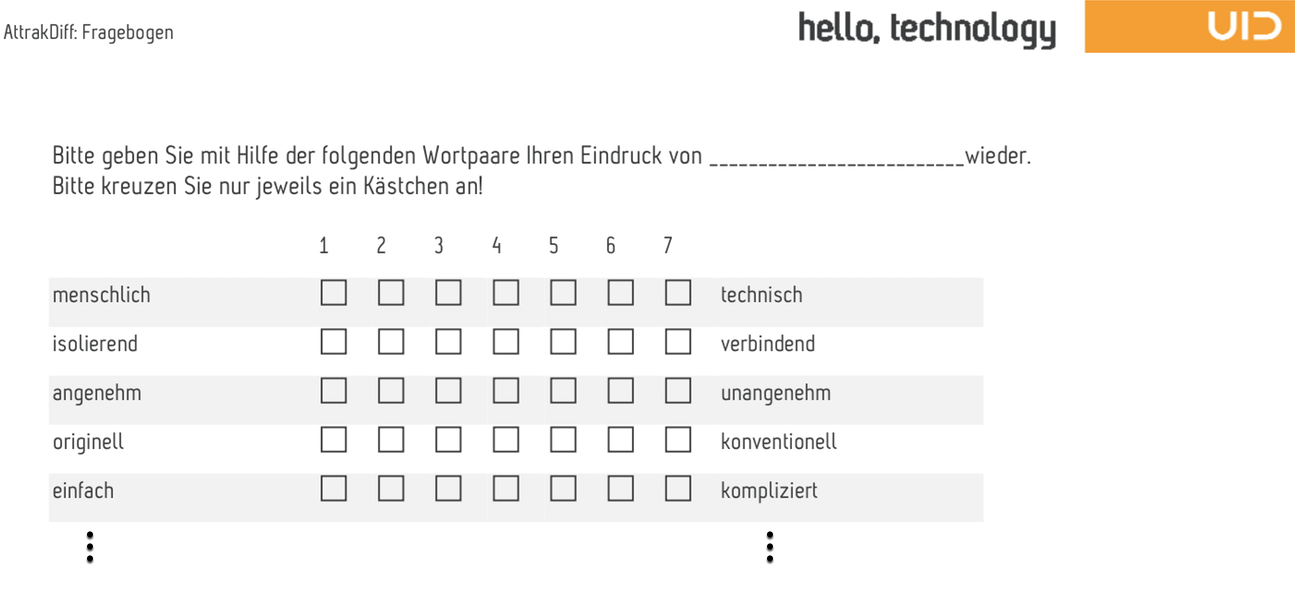
\includegraphics[width=1\textwidth]{files/usa/attrakDiff}
    \caption{AttrakDiff Fragebogen \cite{Anonymous:7qH50iIl}}
    \label{pic:attrakDiff}
\end{figure}




Im Hinblick auf die User Experience kann ein eigener Fragebogen entwickelt werden. So können auch die in Abschnitt \ref{Abschnitt:Kriterienkatalog} aufgestellten Kriterien genauer Hinterfragt und ausgewertet werden. Ein selbst erstellter Fragebogen benötigt einen größeren Zeitaufwand zur Erstellung, denn es wird sowohl Fachwissen als auch Erfahrung benötigt, um die einzelnen Fragen möglichst präzise zu stellen. Zusätzlich zu den konstruierten Fragen sollten auch Kontextinformationen abgefragt werden. Dazu gehören persönliche Informationen wie Alter und Geschlecht, aber auch Fragen nach dem Vorhandensein von bestimmten Geräten, wie PCs oder Smartphones und der Erfahrung im Umgang mit selbigen. \\
Bei der Auswertung der Befragung sollte immer beachtet werden, ob und wie die Befragten selektiert wurden. Jede Befragung, die nur über das Internet durchgeführt wird, kann nur von Nutzern mit Internetzugang wahrgenommen werden. Wird eine Befragung Beispielsweise in einem sozialen Netzwerk durchgeführt, sind Meinungsähnlichkeiten deutlich häufiger. Auf Grund dieser Tatsachen können Fehlinterpretationen entstehen. 

%quantitative Methode
%Usability mit Hilfe eines Fragebogens ermittelt 
%Fragen zu Themen wie „Aufgabenangemessenheit“ oder „Fehlertoleranz“
%anhand einer numerischen Skala beantwor- tet werden. Aus den Antworten werden dann statistische Kennzahlen errechnet, welche einen Vergleich mit vorheri- gen Tests oder Normdaten erlauben.


%Normalerweise kommen vollstandardisierte Fragebögen zum Einsatz, bei denen die Formulierung, die Reihenfolge und das Antwortformat der Fragen fix vorgegeben ist. 

%Es gibt jedoch auch teilstandardisierte Fragebögen, welche neben einer Ratingskala teilweise auch offene Antworten erlauben. So können weitere Details über die Hintergründe einer Bewertung gesammelt werden.

%Grundsätzlich kann für die Usability-Befragung ein beliebi- ger Fragebogen verwendet werden. Die Entwicklung eines eigenen Fragebogens hat zwar den Vorteil, dass auf spe- zifische Punkte eingegangen werden kann, es ist jedoch deutlich zeitaufwändiger und erfordert einiges an Erfah- rung. Deshalb wird in der Regel auf einen standardisierten Usability-Fragebogen zurückgegriffen. Davon sind diverse Varianten mit unterschiedlichen Schwerpunkten und Um- fängen verfügbar. Für die meisten Fragebogen existieren zudem Normdaten, mit denen die Ergebnisse verglichen werden können. Die bekanntesten Fragebogen sind nach- folgend kurz beschrieben.
%Neben den eigentlichen Usability-Fragen ist es Hilfreich, vom Benutzer noch ein paar Kontextinformationen wie Alter, Geschlecht, PC-, oder Produkterfahrung zu erheben, um die Ergebnisse differenzierter auswerten zu können. Einige der Fragebogen enthalten bereits ein Set solcher Fragen.

%unbewusste Se- lektion entstehen, wenn bei einer E-Mail-Befragung nur Benutzer mit einem Internet-Zugang erreicht werden



%
%
%Goms
%
%Goals, Operators, Methods and Selection Rules (GOMS) ist eine analytische Methode zur Vorhersage der Zeit, die ein Benutzer benötigt, um ein gewisses Ziel zu erreichen. Um diese Zeit zu berechnen, wird die Interaktion in elementare Schritte zerlegt und diesen jeweils eine empirisch ermittel- te Zeitwert zugeordnet. Daraus kann dann die benötigte Gesamtzeit aufsummiert werden.
%Die Methode GOMS eignet sich dann, wenn die Effizienz eines Systems ein wichtiger Aspekt ist – beispielsweise für eine Software im Börsenhandel oder in einem Call-Center, bei der es auf jede Sekunde ankommt. Mit der Hilfe von GOMS kann auch sehr einfach die Effizienz von zwei Lö- sungsvarianten miteinander verglichen werden.
%
%
%Die Grundlagen von GOMS
%GOMS wurde von Moran und Newell (1993) entwickelt. Die Methode basiert auf vier verschiedenen Arten von ko- gnitiven Aktivitäten.
%􏰀 Ziele
%Die Ziele sind das, was der Benutzer mit dem Produkt erreichen möchte. Beispielsweise ein Do- kument drucken oder eine Datei löschen.
%􏰀 Operatoren
%Die Operatoren sind atomare Schritte der Wahr- nehmung, Kognition oder Motorik, wie das Drücken einer Taste, das Verstehen einer Ausgabe oder das Warten auf eine Reaktion des Systems.
%􏰀 Methoden
%Die Methoden sind Sequenzen von Operatoren, welche den Benutzer zu seinem Ziel bringen. Oft gibt es für ein Ziel mehrere mögliche Methoden mit unterschiedlichen Operatoren.
%􏰀 Selektionsregeln
%Die Selektionsregeln sind bewusste oder unbe- wusste Regeln, welche dem Benutzer helfen, für ein Ziel eine geeignete Methode zu wählen
%
%
%
%Keystroke Level Model
%Das Keystroke Level Model (KLM) ist eine vereinfachte Variante von GOMS, welche nur Ziele, Operatoren und Methoden verwendet. Sie geht davon aus, dass nach der Formulierung der Ziele die Wahl geeigneter Methoden bereits getroffen ist. Die Methode vernachlässigt zudem, dass Benutzer Fehler machen oder mit der Zeit ermüden.
%KLM-GOMS beschränkt sich auf sechs Operatoren, mit de- nen die komplette Benutzerinteraktion beschrieben wer- den kann. Zur Bestimmung der Gesamtzeit müssen folgen- de Schritte getätigt werden:
%1. Exakte Formulierung des Ziels.
%2. Genaue Beschreibung des Ausgangs- und Endzu- stands des Systems, inklusive der Handpositionen des Benutzers.
%3. Wahl einer Methode, um das Ziel zu erreichen
%4. Zerlegung der Methode in einzelne Operatoren
%5. Einfügen von „Kurz nachdenken“-Operatoren (M), wenn sich der Benutzer mental auf eine Aktion vorbereiten muss.
%6. Summierung der Zeiten zur Gesamtzeit und Multi- plikation mit Altersfaktor:
%
%
%
%%A/B Test 
%
%Der A/B-Test ist eine empirische Methode, bei der zwei Va- rianten einer Lösung miteinander verglichen werden. Dazu werden die Teilnehmer in zwei Untergruppen aufgeteilt. Eine Untergruppe bekommt Variante A gezeigt, die andere Variante B. Anschließend wird durch eine Befragung oder anhand der Konversionsrate verglichen, welche Variante erfolgreicher war. Die Varianten werden normalerweise gleichzeitig gezeigt, um zeitlich bedingte Einflüsse auszu- schließen. Es gibt jedoch auch die Möglichkeit, die Varian- ten hintereinander zu zeigen, mit dem Vorteil, dass keine Infrastruktur für die zufällige Auswahl der beiden Varian- ten benötigt wird.
%A/B-Tests haben ihren Ursprung im Marketing. Dort wer- den für Werbesendungen oft zwei Varianten versandt und anschließend wird ihre Wirkung verglichen. Mit der Verbreitung des Internets sind A/B-Tests jedoch auch für Usability-Tests interessant geworden, da es besonders auf Webseiten sehr einfach zu bewerkstelligen ist, für verschie- dene Benutzer verschiedene Varianten anzuzeigen.
%A/B-Tests sind eine vereinfachte Form sogenannter multi- variater Tests, bei denen jedoch nur eine Variable verän- dert wird. Denn sobald mehrere Variablen verändert wer- den, müssen alle Kombinationen getestet werden, was einen deutlich höheren Aufwand in der Vorbereitung und Auswertung mit sich bringt. Der Testablauf ist jedoch prin- zipiell derselbe.
%A/B-Tests haben gegenüber anderen Methoden den Vor- teil, dass sie das echte Verhalten der Benutzer ohne Verfäl- schung messen. Dabei kommt auch kein Prototyp, sondern eine fertig ausgearbeitete Lösung zum Einsatz. Wenn also eine Variante ein besseres Resultat liefert, ist dies bereits ein realer Erfolg. Um jedoch festzustellen, welches Resul- tat das bessere ist, muss eine Kenngröße definiert werden, an welcher der Erfolg gemessen werden kann. Diese soll- te elektronisch messbar sein. Dies ist in der Praxis jedoch oft schwierig zu erreichen. Nachteilig bei A/B-Tests ist der hohe Aufwand, der für die Ausarbeitung von fertigen Lö-
%sungsvarianten investiert werden muss. Zudem kann pro Test immer nur eine kleine Veränderung untersucht wer- den. A/B-Tests werden daher oft ergänzend zu anderen Evaluationsmethoden eingesetzt.
%Vorbereiten der Varianten
%Als Erstes muss festgelegt werden, welche Veränderungen am Design vorgenommen werden sollen, um die gesetz- ten Ziele zu erreichen. Dazu braucht man eine Hypothese, welche eventuell durch zusätzliche Untersuchungen unter- mauert wird. Wenn es das Ziel wäre, die Anzahl verkauf- ter Produkte pro Besucher eines Webshops zu erhöhen, könnte der Grund ein zu komplizierter Bestellvorgang sein. Deshalb würde dazu vermutlich eine Variante entwickelt, bei der ein Kauf mit weniger Klicks möglich ist.
%Segmentieren der Besucher
%In einem zweiten Schritt müssen die Besucher in zwei Segmente aufgeteilt werden, welche je eine der zwei Lö- sungsvarianten angezeigt bekommen. Die prozentuale Aufteilung kann dabei beliebig gewählt werden. So kön- nen 50% der Besucher die neue Variante testen, oder bei einem vorsichtigen Versuch auch nur 5%. Wichtig ist, dar- auf zu achten, dass für jede Variante eine genügend große Stichprobe erreicht wird, um eine statistisch signifikante Aussage treffen zu können.
%Bestimmen der Referenz
%Um festzustellen, ob die erarbeiteten Lösungsvarianten eine Verbesserung bringen, solle als Erstes eine Messung mit der Originalversion (dem sogenanten Control) vorge- nommen werden. Dadurch wird die Referenz festgelegt. Diese sollte von allen nachfolgenden Varianten nicht mehr unterschritten werden.
%
%
\end{description}

Es wurden sechs verschiedene Methoden dargestellt, mit denen sich die Usability eines Systems ermitteln lässt. Für jede Methode wurde beschrieben, in welchem Entwicklungszyklus sie eingesetzt werden kann. Zusätzlich unterscheiden sich diese Methoden in Aufwand (Zeit und Kosten) und Validität (Aussagekraft).  In Abbildung \ref{pic:AufwandUndVal} werden die einzelnen Methoden in Ellipsenform dargestellt. Im Koordinatensystem kann abgelesen werden, welche Methode aufwändig bzw. weniger Aufwändig ist und welche Methode die genaueren Ergebnisse liefert. Je nach Ziel der Evaluation kann es von Vorteil sein entweder Nutzer, Experten oder beide zu befragen.
\begin{figure}[H]
    \centering
    %trim=left buttom right top
    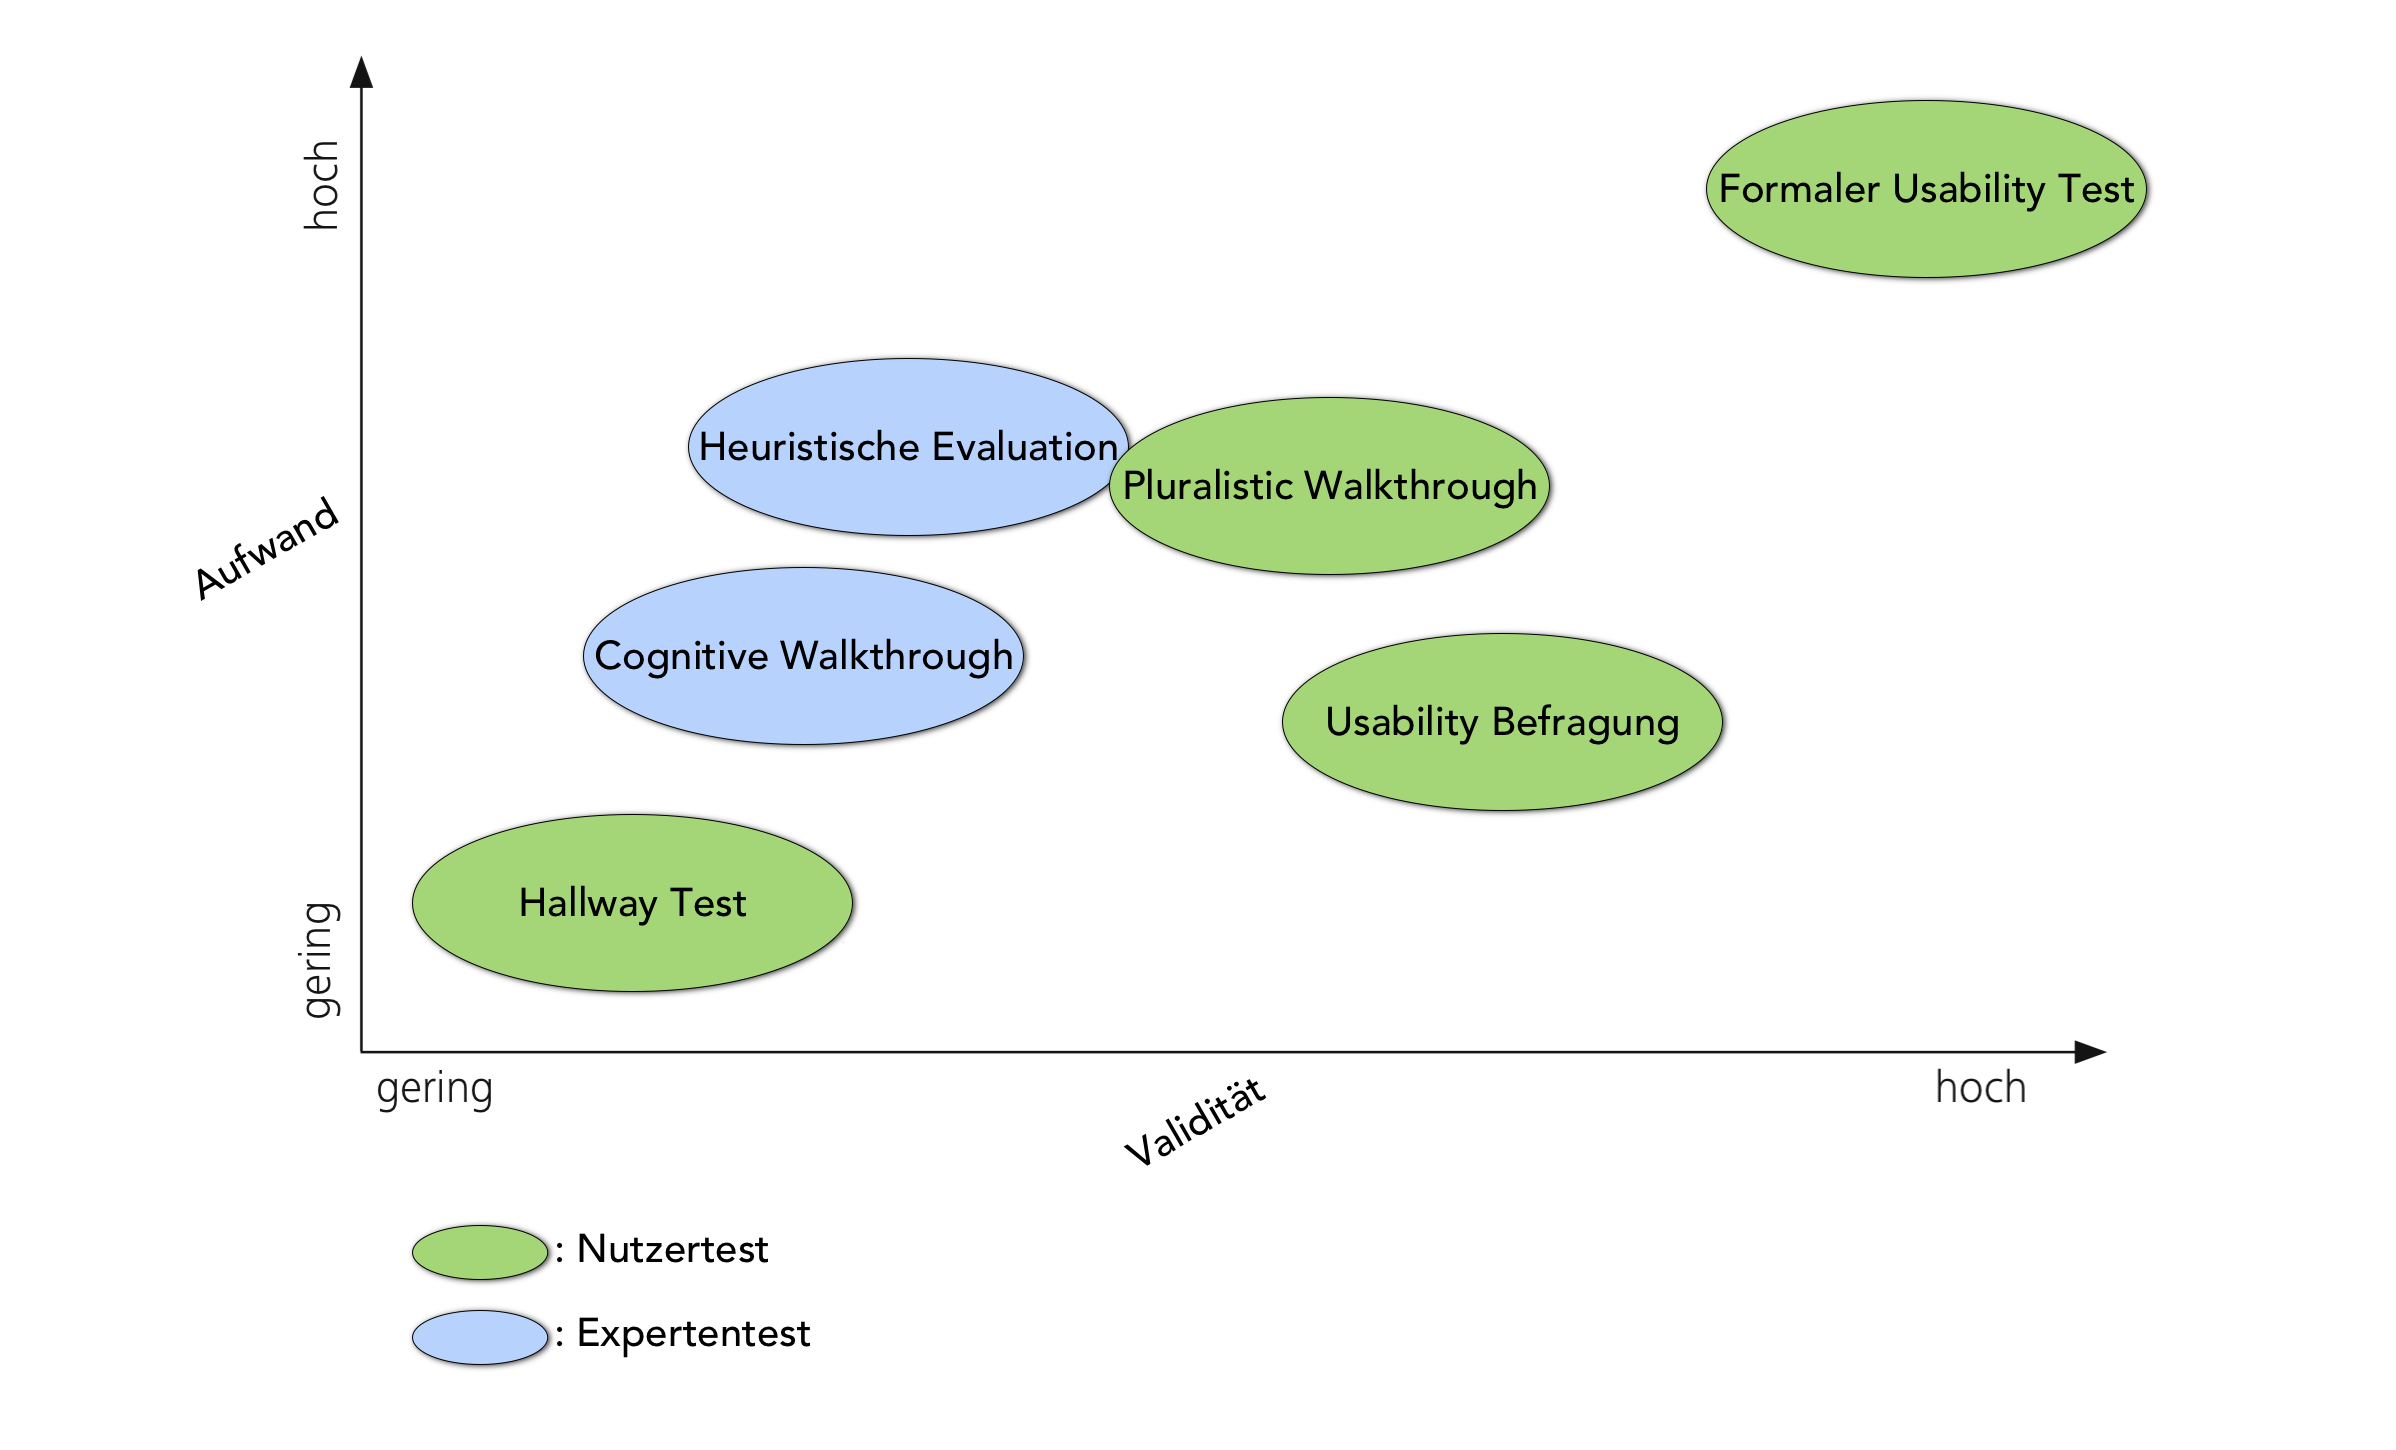
\includegraphics[trim=80 35 90 20,clip,width=1\textwidth]{files/usa/validitaet}
    \caption{Arbeitsaufwand verknüpft mit der Validität der Usability Evaluationsmethoden vlg.  \cite[S. 225]{Moser:2012cn}}
    \label{pic:AufwandUndVal}
\end{figure}
Die vorgestellten Evaluationsmethoden beziehen sich auf Anwendungssoftware. Auch Videospiele sind eine Form von Software. Sie sind somit ein System, dessen User Experience durch die in diesem Kapitel vorgestellten Kriterien und Evaluationsmethoden ermittelt werden könnte. Videospiele sind aber zusätzlich \textit{Spiele}. \\
Anwendungssoftware, die eine gute User Experience bietet ist darauf ausgelegt Aufgaben effizient und angenehm mit dem Nutzer zu lösen. Er sollte im Idealfall nicht stark beansprucht werden und die Aufgaben schnell lösen können. Spiele sind aber darauf ausgelegt ihre Spieler zu fordern. So gibt es einen grundlegenden Unterschied in diesen beiden System. \\
Videospiele können sich zusätzlich an einer Vielzahl multimedialer Inhalte bedienen. Allein diese Inhalte können bei Personen Emotionen hervorrufen. Es muss somit weitere Aspekte geben die die User Experience im Bezug auf Videospiele beeinflussen.
